\documentclass{article}
\PassOptionsToPackage{numbers}{natbib}
\usepackage[final]{neurips_2019}
\usepackage[utf8]{inputenc}
\usepackage[T1]{fontenc}
\usepackage{hyperref}
\hypersetup{hidelinks}
\usepackage{url}
\usepackage{booktabs}
\usepackage{amsmath}
\usepackage{amsfonts}
\usepackage{nicefrac}
\usepackage{microtype}
\usepackage{graphicx}
\usepackage{xcolor}
\usepackage{xparse}
\usepackage{array}
\usepackage{float}
\setlength{\textfloatsep}{7pt plus 1pt minus 1pt}
\setlength{\intextsep}{6pt plus 1pt minus 1pt}

% Columbia COMS 4705 Project Milestone template; instructions intentionally removed.
% Numbers below come from ../results/ (results_log.csv, summary.csv,
% paired_differences.csv, confusable_pairs_test.csv; run of 2026-11-22).
\NewDocumentCommand{\projecttitle}{m m m}{%
  \title{#1\\[0.7em]
  {\normalsize\normalfont Columbia COMS 4705 Project Milestone}\\[0.8em]
  \parbox{0.95\textwidth}{\normalfont\small\centering
    \textbf{Keywords:} \textit{#2}\par\vspace{0.4em}
    \textbf{TA Mentor:} #3\par}}%
}
\projecttitle
  {Few-Shot Banking Customer Intent Classification: A Controlled Study of SetFit}
  {intent detection, few-shot classification, contrastive learning, SetFit}
  {Rishika Mamidibathula}

\author{
  Tian Zhou \\
  Columbia University \\
  \texttt{tz2751@columbia.edu}
  \And
  Liping Zhu \\
  Columbia University \\
  \texttt{lz3147@columbia.edu}
  \And
  Jim Lu \\
  Columbia University \\
  \texttt{yl6325@columbia.edu}
}

\begin{document}
\maketitle

\begin{abstract}
We study whether SetFit's pairwise representation adaptation improves fine-grained banking intent detection enough to justify its cost. On BANKING77 with 8 and 32 examples per intent, we compare SetFit with frozen embeddings plus logistic regression (Frozen+LR) and cross-entropy (CE) tuning from the same encoder and samples. Over three paired seeds, SetFit (78.6/87.1 test macro-F1) matches but does not beat Frozen+LR (78.8/87.3) at 26--37$\times$ its training time; both beat CE (70.6/83.6). SetFit's validation score peaks at its first checkpoint in every final run, which our next experiments examine.
\end{abstract}

\section{Approach}
\textbf{Task and motivation.} BANKING77 is 77-way, single-label English classification of banking support requests \citep{casanueva2020efficient,polyai2020banking77}. SetFit learns from same/different-label sentence pairs \citep{tunstall2022setfit}, while frozen sentence encoders can already work well for intent detection \citep{ma2022sentence}. We ask whether adaptation beats a matched frozen encoder consistently across samples and at acceptable cost, notably on confusable labels \citep{zhang2025clear}.

\textbf{Matched methods.} All methods start from \texttt{all-MiniLM-L6-v2} (22.7M parameters; 384-dimensional, mean-pooled, normalized embeddings) \citep{minilm2026}. (1) \textbf{Frozen+LR} freezes the encoder and fits multinomial logistic regression (LR). (2) \textbf{CE tuning} jointly trains the encoder and a 77-way linear head with cross-entropy. (3) \textbf{SetFit} updates the encoder with balanced positive/negative sentence pairs, re-embeds the selected labeled texts, then fits the \emph{same} LR configuration as Frozen+LR. Its pair objective is
\begin{equation}
  \mathcal{L}_{\mathrm{pair}}=\frac{1}{B}\sum_{i=1}^{B}
  \bigl[\cos(f_{\theta}(x_i),f_{\theta}(x'_i))-z_i\bigr]^2,
  \qquad z_i=\mathbf{1}[y_i=y'_i].
\end{equation}
For each anchor, we draw four distinct positive and four distinct negative partners from the selected training set. Both LR models use \texttt{lbfgs}, $C=1$, intercept, and 2,000 maximum iterations; CE is compared at the pipeline level.

\textbf{Implementation (complete).} We wrote all code in PyTorch \citep{paszke2019pytorch} and \texttt{transformers} \citep{wolf2020transformers}: the encoder (masked mean pooling, L2 normalization), pair sampler, training loops, checkpoint selection, and per-component timing. SetFit's code \citep{setfit2026} served only as a reference; LR and metrics use scikit-learn \citep{pedregosa2011scikit}. Eight offline tests on synthetic data cover every stage; all 32 runs share one code hash.

\section{Experiments}
\textbf{Data.} Our exact-text audit of BANKING77's 10,003 training and 3,080 test texts \citep{casanueva2020efficient,polyai2020banking77} removes 4 redundant training rows and 6 training texts also found in test (9,993 remain; test is untouched). Stratified validation (seed 2026) takes 965 examples, leaving 9,028 candidates ($\geq$32 per intent); nested samples have 616/2,464 texts (4,928/19,712 SetFit pairs) at $k=8/32$.

\textbf{Protocol and metrics.} Seed 0 selects each tuned method's learning rate ($10^{-5}$ vs.\ $3\times10^{-5}$) on validation; final runs on seeds 11, 22, and 33 share each training sample across methods and are scored once on test. Encoder training: AdamW (weight decay 0.01), batch 32 (sentences for CE, pairs for SetFit), clipping 1.0, 10\% warmup then linear decay, FP16, 128-token truncation (never triggered), 300/1,000-update caps, validation every 50/100, best validation macro-F1 checkpoint kept. Test macro-F1 (unweighted mean of the 77 per-class F1s) is primary and accuracy secondary.

\begin{table}[H]
\centering
\caption{Final test results, seeds 11/22/33 (mean $\pm$ sample SD). $\Delta$: paired macro-F1 difference from Frozen+LR in points (negative on every seed). Time includes checkpoint-time evaluation.}
\label{tab:models}
\small
\begin{tabular}{@{}lcccccc@{}}
\toprule
& \multicolumn{2}{c}{Test macro-F1 (\%) $\uparrow$} & \multicolumn{2}{c}{$\Delta$ vs.\ Frozen+LR} & \multicolumn{2}{c}{Train time (s) $\downarrow$} \\
\cmidrule(lr){2-3}\cmidrule(lr){4-5}\cmidrule(l){6-7}
Method & 8-shot & 32-shot & 8-shot & 32-shot & 8-shot & 32-shot \\
\midrule
Frozen+LR & \textbf{78.8} $\pm$ 0.3 & \textbf{87.3} $\pm$ 0.2 & -- & -- & 0.7 $\pm$ 0.3 & 1.7 $\pm$ 0.6 \\
CE tuning & 70.6 $\pm$ 1.5 & 83.6 $\pm$ 0.2 & $-8.2$ & $-3.7$ & 12.2 $\pm$ 0.6 & 37.6 $\pm$ 0.4 \\
SetFit & 78.6 $\pm$ 0.2 & 87.1 $\pm$ 0.2 & $-0.20$ & $-0.15$ & 18.0 $\pm$ 0.6 & 63.6 $\pm$ 0.7 \\
\bottomrule
\end{tabular}
\end{table}

\textbf{Main result.} SetFit does not beat Frozen+LR (Table~\ref{tab:models}). Its paired difference is negative on all six seed--size pairs but at most 0.3 points, which with three seeds we read as no gain; accuracy agrees (79.6/87.3 vs.\ 79.8/87.4). It needs 26$\times$/37$\times$ Frozen+LR's training time and 2.5--2.6$\times$ its peak GPU memory (889/983 vs.\ 349/372 MB). We expected a gain, since SetFit targets this few-shot regime \citep{tunstall2022setfit}.

\textbf{Training curves (Figure~\ref{fig:curves}).} In every final SetFit run the first checkpoint (update 50/100) is best; later ones score lower although the pair loss falls (32 shots: 86.0--86.6 at update 100, 82.7--84.6 at 1,000). In five of six runs it already trails Frozen+LR on validation, and update 0 (equal to Frozen+LR) is never evaluated. Either \texttt{all-MiniLM-L6-v2}, already trained contrastively on over a billion sentence pairs \citep{minilm2026}, leaves little to gain (as \citep{ma2022sentence} suggest), or useful adaptation ends before the first checkpoint.

\textbf{CE tuning (change since the proposal).} With the head at the encoder's rate, as proposed, CE's loss fell only from $\ln 77\approx4.34$ to 4.09/3.89, with best seed-0 validation macro-F1 59.7/84.2. We gave the random head its own untuned rate of $10^{-3}$, re-ran both encoder rates, and locked $3\times10^{-5}$ for both sizes (validation 70.6/84.0; 84.2 without it at 32 shots), so CE had twice SetFit's tuning runs. Its last 200 updates at 32 shots added at most 0.8 points, so a longer budget is unlikely to close its 3.6-point gap to SetFit.

\textbf{Cost accounting (TA feedback).} At 32 shots, SetFit's 63.6\,s include 39.1\,s of updates, 15.0\,s for 10 checkpoint LR fits, 5.0\,s checkpoint re-embedding, 2.9\,s validation, and 1.4\,s final refit, so checkpoint selection is 36\% of its cost (31\% at 8 shots). All 32 runs trained in 12.7 minutes on one NVIDIA L4.

\textbf{Variation and errors (TA feedback).} Frozen+LR has no optimizer randomness, so its 8-shot range (78.5--79.1) reflects the training sample alone (SetFit 78.4--78.9, CE 69.2--72.2); it is wider than SetFit's per-seed differences, which never change sign. On five confusable pairs preselected on seed-0 Frozen+LR validation, pooled test confusion is 13.8/13.6/15.3\% (SetFit/Frozen+LR/CE) at 8 shots and 7.5/7.1/9.2\% at 32. Whether SetFit helps a pair depends on the sample: at 8 shots, 4 of 5 pairs improve on one seed and worsen on another (by $\leq$2 of 80 examples). On seed 11 (8 shots), SetFit fixes 59 Frozen+LR errors and adds 65. In the first cases drawn (seed 2026), it fixes ``I need a new PIN'' (Frozen+LR: \texttt{get\_physical\_card}) but breaks ``Please tell me about SWIFT transfers at this bank'' (\texttt{top\_up\_by\_bank\_transfer\_charge}$\,\to\,$\texttt{transfer\_into\_account}).

\section{Future Work}
\textbf{Changes and plan.} Besides CE's head learning rate, core runs finished on Nov.~22, not Dec.~5, freeing time for (i)--(iii) under the locked protocol. (i) \emph{Checkpoint grid}: add update 0 and validate every 10 updates up to 100 (Nov.~30). (ii) \emph{Encoder ablation}: rerun all methods from the base model of \texttt{all-MiniLM-L6-v2} (same architecture, no contrastive sentence training \citep{minilm2026}); if headroom is the cause, SetFit should then beat Frozen+LR (Dec.~5). (iii) \emph{CE check}: a 2,000-update 32-shot cap, not used for selection. (iv) \emph{Error analysis (TA feedback)}: label the 40 drawn seed-11 cases (ten per correctness cell) as close-label ambiguity, paraphrase, or missing information, and add per-class recall (Dec.~12). Stretch: hard negatives (a proposal option), $k\in\{2,4\}$. Final report: Dec.~17.

\clearpage
\begin{figure}[H]
\centering
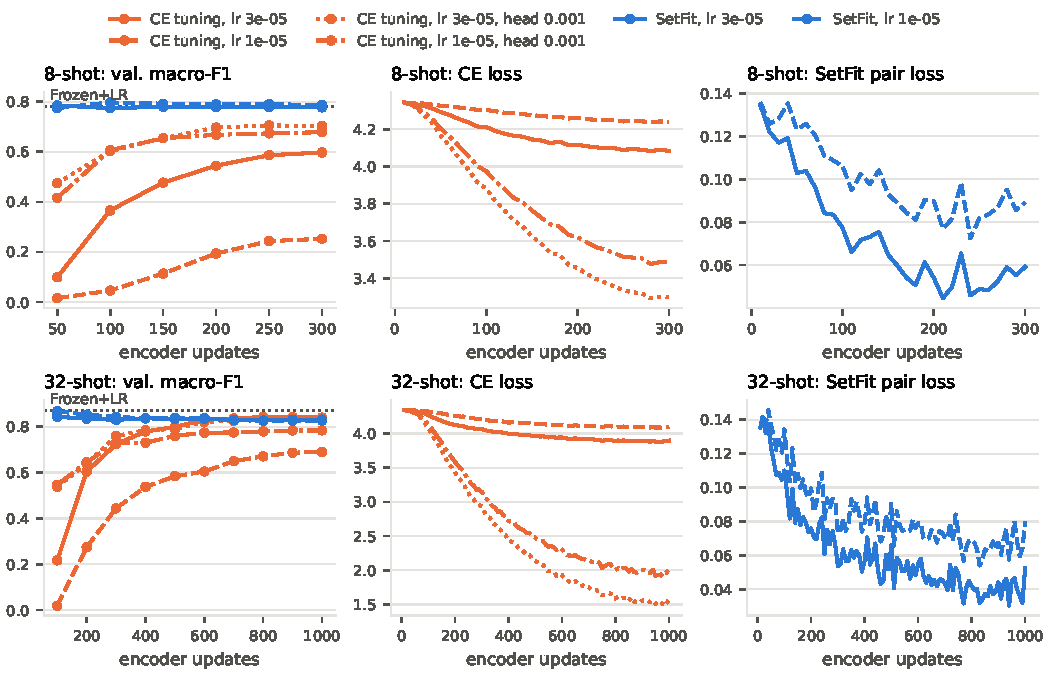
\includegraphics[width=\textwidth]{figures/tuning_curves.pdf}
\caption{Seed-0 tuning runs (validation only; the final seeds show the same pattern). Left: validation macro-F1 per checkpoint, with Frozen+LR as the dotted line. Middle: CE training loss; dotted and dash-dot lines use the separate head learning rate $10^{-3}$. Right: SetFit pair loss. SetFit's pair loss keeps falling while its validation macro-F1 stays near the Frozen+LR line.}
\label{fig:curves}
\end{figure}

\bibliographystyle{unsrt}
\bibliography{references}
\end{document}
